\documentclass[10pt]{article}
\usepackage[usenames]{color} %used for font color
\usepackage{amssymb} %maths
\usepackage{amsmath} %maths
\usepackage[utf8]{inputenc} %useful to type directly diacritic characters
\begin{document}
L'interface de la station de base est plutôt simple comme le démontre la figure suivante \ref{f:InterfaceImage}. Elle a comme particularité d'afficher une image virtuelle la plus semblable possible à l'image perçue par la CameraMonde.
\medbreak

\begin{figure}[htp]
   \centering
   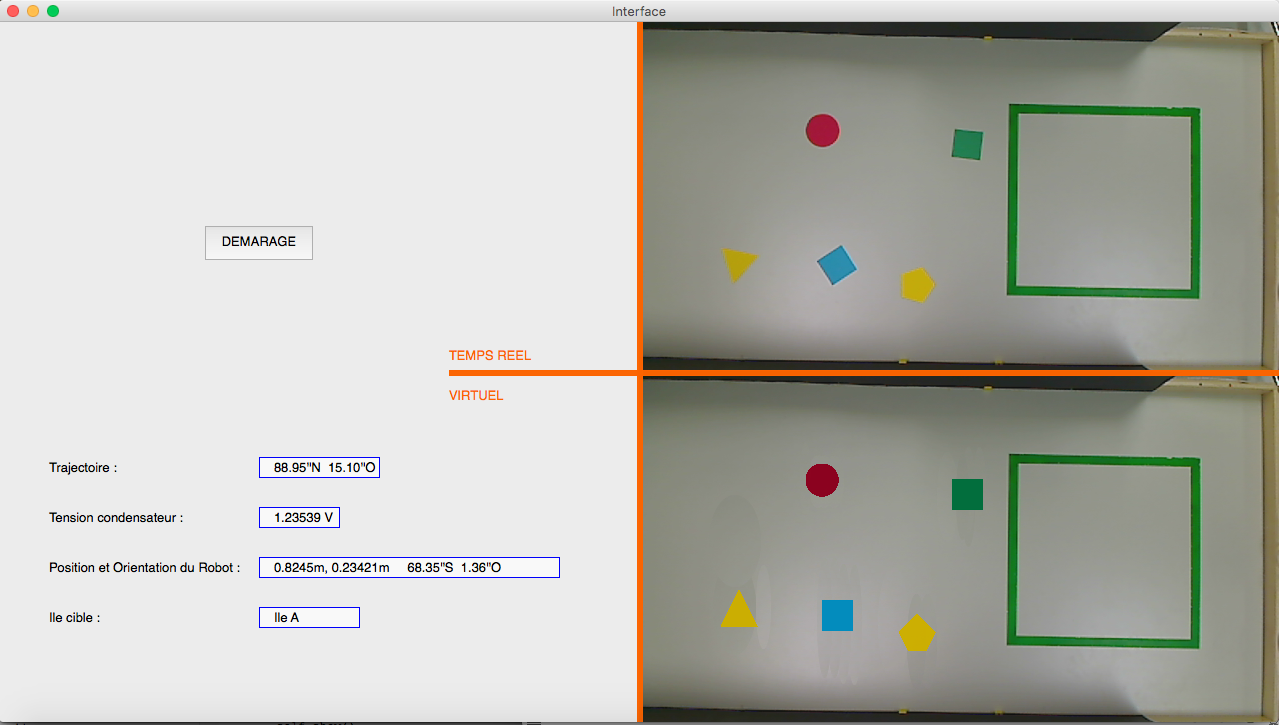
\includegraphics[width=1\textwidth]{fig/interface_Image.png}
   \caption{Interface de la Station}
   \label{f:InterfaceImage}
\end{figure}

\medbreak
La section gauche de l'interface nous donne des informations plutôt simples sur le démarage de la chasse au trésor en général. Elle affiche également des informations pertinentes sur le robot comme l'île cible, l'orientation, la position et la direction du robot ainsi que la tension dans le condensateur.
\medbreak
Pour l'instant, l'interface n'est pas connectée au système, mais elle est plutôt prêt à recevoir des commandes tel que la position, la forme et la couleur d'un objet pour la reproduire de façon plutôt similaire dans notre image virtuelle comme le démontre la partie inférieure droite de l'interface.
\medbreak
Le point fort de l'interface est l'idée d'utiliser une photo de la CaméraMonde avant que les objets soient insérés ou que le robot soit inséré pour ensuite ajouter des objets virtuellement. Celà nous aidera beaucoup plus à savoir si notre système saisi bien les formes, les emplacements et les couleurs de toutes sortes à l'oeil nu. On devrait obtenir une image semblable la figure \ref{f:InterfaceImage} précédente dans la section virtuelle en bas à droite. On constate sur la figure que l'image en temps réel est très semblable à sa reproduction.

La forme et la couleur sur le dessus du robot pour pouvoir bien déterminer l'orientation et la position du robot n'ont toujours pas été déterminées. Par contre, lorsqu'elle sera déterminé. Il sera nécessaire de l'afficher avec une bonne orientation (contrairement aux objets sur la map, bien qu'il serait intéressant également de reproduire des objets dans leurs bons angles.)
\medbreak

 Il sera intéressant aussi potentiellement d'afficher la trajectoire du robot sur la map virtuelle. Pour voir s'il suit bien sa trajectoire pour des tests. Et également un bouton stop pour arrêter les opérations du robot. Ceci nous permettrait de perdre moins de temps lorsqu'on voit qu'il y a quelque chose qui ne marche pas dans les commandes du robot et de la station de base.
\end{document}